\chapter{Functions: The Morphisms of Mathematics}

\section{From Relations to Functions}

\begin{intuition}
Relations are general correspondences---an element of $A$ can relate to zero, one, or many elements of $B$.

But most mathematical structures require something more specific: each input should produce \textit{exactly one} output.

Think of:
\begin{itemize}
    \item $f(x) = x^2$ --- each number has exactly one square
    \item Temperature at a location --- each point has one temperature
    \item The derivative $\frac{d}{dx}$ --- each (differentiable) function has one derivative
\end{itemize}

This ``one input, one output'' property defines a \textbf{function}.
\end{intuition}

\begin{historicalnote}
The word ``function'' comes from Leibniz (1673), meaning a quantity depending on a variable. 

But the modern definition---function as a set of ordered pairs---emerged slowly:
\begin{itemize}
    \item \textbf{18th century}: Functions were formulas ($y = x^2 + 3x$)
    \item \textbf{Dirichlet (1837)}: Functions as arbitrary correspondences (not just formulas)
    \item \textbf{Dedekind (1888)}: Functions as single-valued relations
    \item \textbf{Bourbaki (1939)}: Functions as special subsets of Cartesian products
\end{itemize}

This evolution mirrors mathematics' shift from computation to abstraction.
\end{historicalnote}

\section{The Formal Definition}

\begin{definition}[Function]
Let $A$ and $B$ be sets. A \textbf{function} $f$ from $A$ to $B$ (written $f: A \to B$) is a relation $f \subseteq A \times B$ satisfying:

\begin{enumerate}
    \item \textbf{Existence (Totality)}: $\forall x \in A, \exists y \in B, (x, y) \in f$
    
    (Every element of $A$ has at least one image)
    
    \item \textbf{Uniqueness (Single-valued)}: $\forall x \in A, \forall y_1, y_2 \in B, ((x, y_1) \in f \land (x, y_2) \in f) \implies y_1 = y_2$
    
    (Every element of $A$ has at most one image)
\end{enumerate}

We write $f(x) = y$ to mean $(x, y) \in f$.
\end{definition}

egin{center}
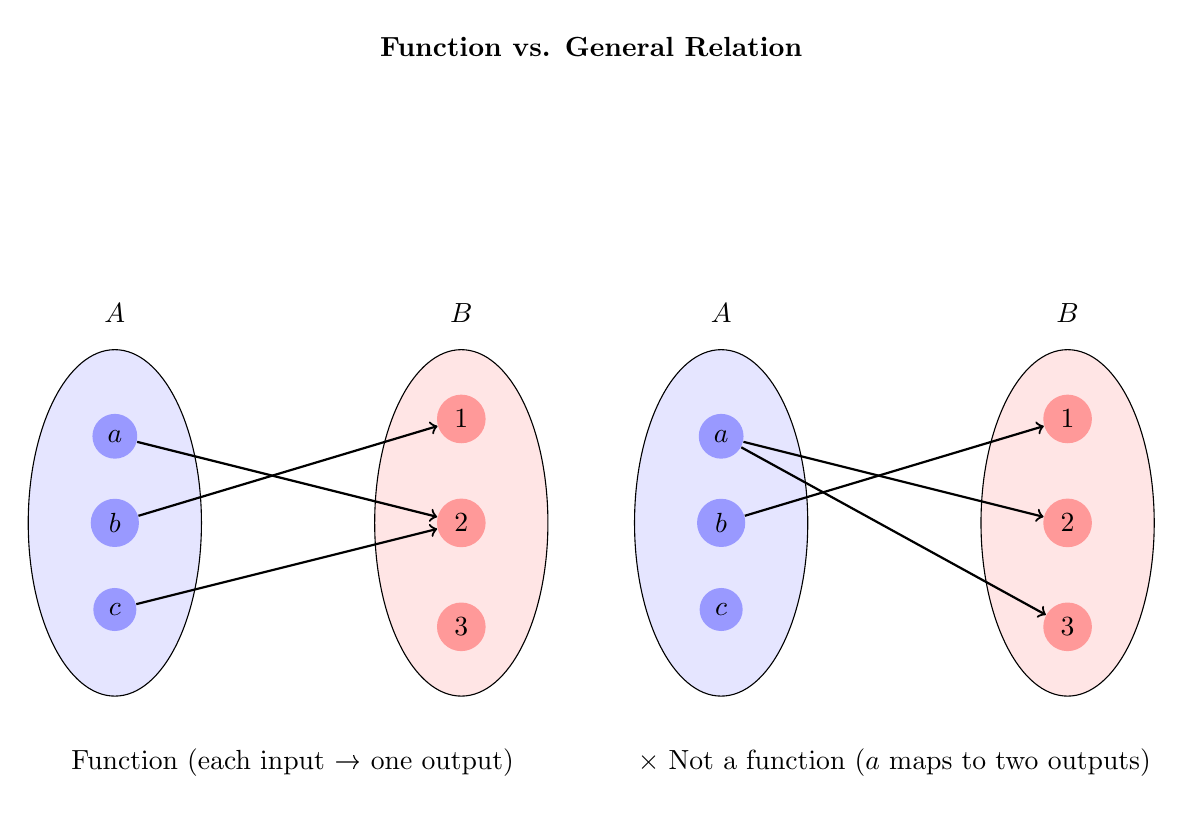
\begin{tikzpicture}[scale=1.1]
    \node at (5.5, 5.5) {\textbf{Function vs. General Relation}};
    
    % Function
    \begin{scope}[shift={(0,0)}]
        \draw[fill=blue!10] (0,0) ellipse (1cm and 2cm);
        \draw[fill=red!10] (4,0) ellipse (1cm and 2cm);
        \node[above] at (0,2.2) {$A$};
        \node[above] at (4,2.2) {$B$};
        
        \node[circle, fill=blue!40] (a1) at (0,1) {$a$};
        \node[circle, fill=blue!40] (a2) at (0,0) {$b$};
        \node[circle, fill=blue!40] (a3) at (0,-1) {$c$};
        
        \node[circle, fill=red!40] (b1) at (4,1.2) {$1$};
        \node[circle, fill=red!40] (b2) at (4,0) {$2$};
        \node[circle, fill=red!40] (b3) at (4,-1.2) {$3$};
        
        \draw[->, thick] (a1) -- (b2);
        \draw[->, thick] (a2) -- (b1);
        \draw[->, thick] (a3) -- (b2);
        
        \node[below] at (2, -2.5) {$\checkmark$ Function (each input → one output)};
    \end{scope}
    
    % NOT a function
    \begin{scope}[shift={(7,0)}]
        \draw[fill=blue!10] (0,0) ellipse (1cm and 2cm);
        \draw[fill=red!10] (4,0) ellipse (1cm and 2cm);
        \node[above] at (0,2.2) {$A$};
        \node[above] at (4,2.2) {$B$};
        
        \node[circle, fill=blue!40] (a1) at (0,1) {$a$};
        \node[circle, fill=blue!40] (a2) at (0,0) {$b$};
        \node[circle, fill=blue!40] (a3) at (0,-1) {$c$};
        
        \node[circle, fill=red!40] (b1) at (4,1.2) {$1$};
        \node[circle, fill=red!40] (b2) at (4,0) {$2$};
        \node[circle, fill=red!40] (b3) at (4,-1.2) {$3$};
        
        \draw[->, thick] (a1) -- (b2);
        \draw[->, thick] (a1) -- (b3);
        \draw[->, thick] (a2) -- (b1);
        
        \node[below] at (2, -2.5) {$\times$ Not a function ($a$ maps to two outputs)};
    \end{scope}
\end{tikzpicture}
\end{center}

\begin{keyidea}
A function is uniquely determined by its \textbf{graph}:
\[\text{graph}(f) = \{(x, f(x)) : x \in A\} \subseteq A \times B\]

In set theory, the function \textit{is} its graph. There's no distinction between $f$ and graph$(f)$.

When we write $f: A \to B$, we're declaring:
\begin{itemize}
    \item $f$ is a subset of $A \times B$
    \item $A$ is the domain (set of all inputs)
    \item $B$ is the codomain (set where outputs live)
    \item Each $x \in A$ appears in exactly one pair $(x, y) \in f$
\end{itemize}
\end{keyidea}

\begin{remark}[Connecting Set-Theoretic and ``Rule-Based'' Notation]
There is often confusion between the formal definition of functions as sets of ordered pairs and the familiar notation like ``$f(x) = x^2$.'' Let us clarify this explicitly.

\textbf{The Set-Theoretic Object:}

When we say $f: \mathbb{R} \to \mathbb{R}$ is a function, we mean:
\[f \subseteq \mathbb{R} \times \mathbb{R}\]
is a subset (specifically, a relation) satisfying totality and uniqueness. The function $f$ is literally this set of ordered pairs.

\textbf{The Notation $f(x)$:}

When we write $f(x) = x^2$, we mean:
\begin{itemize}
    \item $f(x)$ denotes the \textbf{unique value} $y$ such that $(x, y) \in f$
    \item The equation $f(x) = x^2$ is a \textbf{rule} specifying which pairs belong to $f$
    \item More precisely: $f = \{(x, x^2) : x \in \mathbb{R}\}$
\end{itemize}

\textbf{Distinguishing $f$ from $f(x)$:}

This is crucial but often glossed over:
\begin{itemize}
    \item $f$ is the \textbf{function itself} (an object, a set)
    \item $f(x)$ is the \textbf{value} the function assigns to the input $x$ (an element of the codomain)
\end{itemize}

For example:
\begin{itemize}
    \item $f = \{(1, 1), (2, 4), (3, 9)\}$ is a function (a set of three pairs)
    \item $f(2) = 4$ is a number (the output when input is 2)
    \item $f$ is one object; $f(2)$ is another object (its value at 2)
\end{itemize}

\textbf{Why We Use Both:}

\begin{itemize}
    \item The set-theoretic definition ($f \subseteq A \times B$) is rigorous and unambiguous. It allows us to prove theorems about functions using only set theory.
    
    \item The rule notation ($f(x) = \cdots$) is convenient for specifying and computing with functions. It mirrors how functions are used in practice.
\end{itemize}

Both perspectives coexist:
\begin{itemize}
    \item When we prove general theorems, we think of $f$ as a subset of $A \times B$
    \item When we define specific functions, we write $f(x) = $ some expression
    \item The bridge: writing $f(x) = y$ is shorthand for $(x, y) \in f$
\end{itemize}

\textbf{Example---The Squaring Function:}

Consider $f: \mathbb{R} \to \mathbb{R}$ defined by $f(x) = x^2$.

\begin{itemize}
    \item \textit{Set-theoretically}: $f = \{(x, x^2) : x \in \mathbb{R}\} \subseteq \mathbb{R} \times \mathbb{R}$
    \item \textit{As a rule}: For any $x \in \mathbb{R}$, the value $f(x)$ is computed as $x^2$
    \item \textit{Evaluation}: $f(3) = 9$ means $(3, 9) \in f$
    \item \textit{The function}: $f$ is the entire infinite set of pairs, not just one value
\end{itemize}

This dual perspective---function as set, function as rule---is fundamental to modern mathematics. The set-theoretic foundation ensures rigor; the rule-based notation ensures usability.
\end{remark}

\subsection{Domain, Codomain, and Image}

\begin{definition}
Let $f: A \to B$ be a function.

\begin{itemize}
    \item The \textbf{domain} of $f$ is $A$ (set of all valid inputs)
    
    \item The \textbf{codomain} of $f$ is $B$ (target set where outputs are allowed)
    
    \item The \textbf{image} (or range) of $f$ is:
    \[\text{Im}(f) := \{y \in B : \exists x \in A, f(x) = y\} = \{f(x) : x \in A\}\]
    
    (The subset of $B$ actually reached by $f$)
\end{itemize}

Note: $\text{Im}(f) \subseteq B$, but equality need not hold.
\end{definition}

\begin{warning}
\textbf{Codomain vs. Image}

These are often confused!

\begin{itemize}
    \item \textbf{Codomain}: Where outputs are \textit{allowed} to be (specified in definition)
    \item \textbf{Image}: Where outputs \textit{actually} are (computed from function)
\end{itemize}

Example: $f: \mathbb{R} \to \mathbb{R}$ defined by $f(x) = x^2$
\begin{itemize}
    \item Codomain = $\mathbb{R}$ (all reals)
    \item Image = $[0, \infty)$ (only non-negative reals)
\end{itemize}

Changing the codomain changes the function! 

$f_1: \mathbb{R} \to \mathbb{R}$ and $f_2: \mathbb{R} \to [0, \infty)$ with the same formula $f(x) = x^2$ are \textit{different functions} (same graph, different codomains).
\end{warning}

\begin{example}
Let $f: \{1, 2, 3\} \to \{a, b, c, d\}$ be defined by:
\[f = \{(1, a), (2, c), (3, c)\}\]

Then:
\begin{itemize}
    \item Domain: $\{1, 2, 3\}$
    \item Codomain: $\{a, b, c, d\}$
    \item Image: $\{a, c\}$ (elements $b$ and $d$ are not reached)
\end{itemize}
\end{example}

\section{Types of Functions: Injections, Surjections, Bijections}

Functions can be classified by how they map domain to codomain.

\subsection{Injective Functions (One-to-One)}

\begin{intuition}
An injective function never ``collides''---distinct inputs always produce distinct outputs.

Think of assigning student ID numbers: each student gets a unique ID. No two students share an ID.
\end{intuition}

\begin{definition}[Injection]
A function $f: A \to B$ is \textbf{injective} (or \textbf{one-to-one}) if:
\[\forall x_1, x_2 \in A, (f(x_1) = f(x_2) \implies x_1 = x_2)\]

Equivalently (contrapositive):
\[\forall x_1, x_2 \in A, (x_1 \neq x_2 \implies f(x_1) \neq f(x_2))\]
\end{definition}

egin{center}
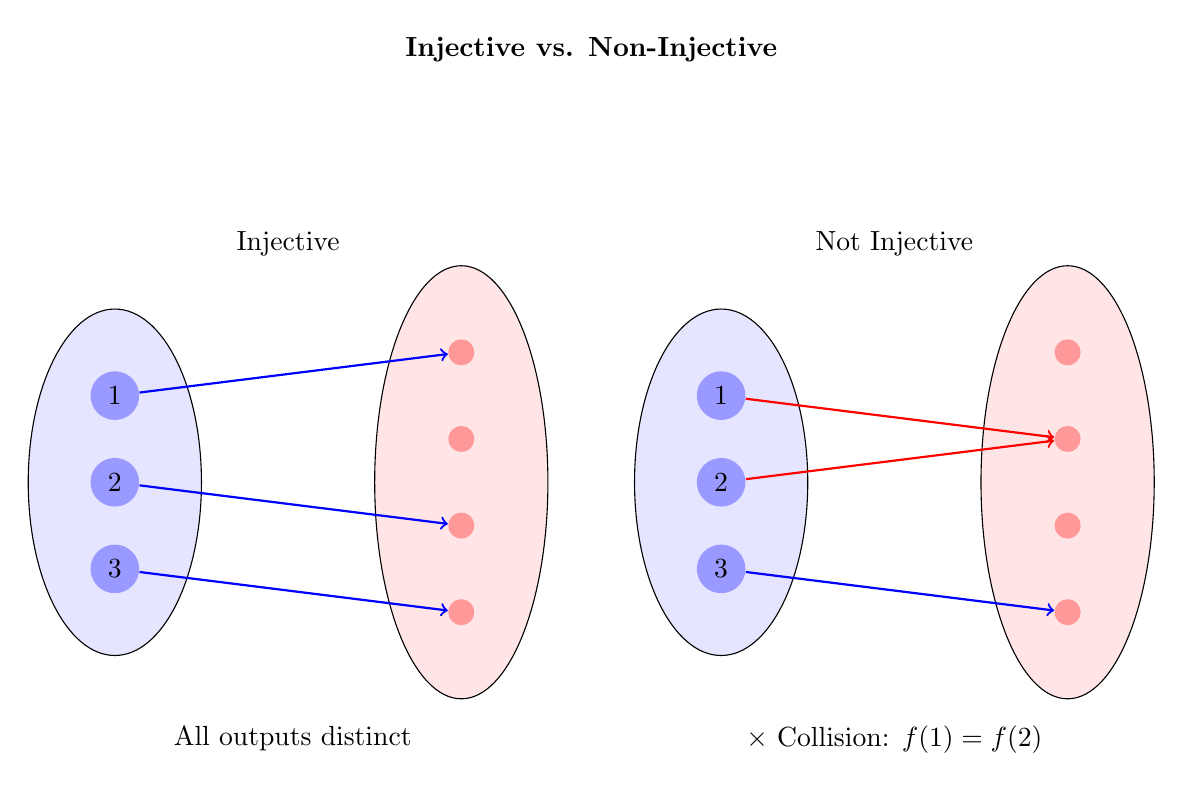
\begin{tikzpicture}[scale=1.1]
    \node at (5.5, 5) {\textbf{Injective vs. Non-Injective}};
    
    % Injective
    \begin{scope}[shift={(0,0)}]
        \draw[fill=blue!10] (0,0) ellipse (1cm and 2cm);
        \draw[fill=red!10] (4,0) ellipse (1cm and 2.5cm);
        \node[above] at (2,2.5) {Injective};
        
        \node[circle, fill=blue!40] (a1) at (0,1) {$1$};
        \node[circle, fill=blue!40] (a2) at (0,0) {$2$};
        \node[circle, fill=blue!40] (a3) at (0,-1) {$3$};
        
        \node[circle, fill=red!40] (b1) at (4,1.5) {};
        \node[circle, fill=red!40] (b2) at (4,0.5) {};
        \node[circle, fill=red!40] (b3) at (4,-0.5) {};
        \node[circle, fill=red!40] (b4) at (4,-1.5) {};
        
        \draw[->, thick, blue] (a1) -- (b1);
        \draw[->, thick, blue] (a2) -- (b3);
        \draw[->, thick, blue] (a3) -- (b4);
        
        \node[below] at (2, -2.7) {$\checkmark$ All outputs distinct};
    \end{scope}
    
    % Non-injective
    \begin{scope}[shift={(7,0)}]
        \draw[fill=blue!10] (0,0) ellipse (1cm and 2cm);
        \draw[fill=red!10] (4,0) ellipse (1cm and 2.5cm);
        \node[above] at (2,2.5) {Not Injective};
        
        \node[circle, fill=blue!40] (a1) at (0,1) {$1$};
        \node[circle, fill=blue!40] (a2) at (0,0) {$2$};
        \node[circle, fill=blue!40] (a3) at (0,-1) {$3$};
        
        \node[circle, fill=red!40] (b1) at (4,1.5) {};
        \node[circle, fill=red!40] (b2) at (4,0.5) {};
        \node[circle, fill=red!40] (b3) at (4,-0.5) {};
        \node[circle, fill=red!40] (b4) at (4,-1.5) {};
        
        \draw[->, thick, red] (a1) -- (b2);
        \draw[->, thick, red] (a2) -- (b2);
        \draw[->, thick, blue] (a3) -- (b4);
        
        \node[below] at (2, -2.7) {$\times$ Collision: $f(1) = f(2)$};
    \end{scope}
\end{tikzpicture}
\end{center}

\begin{theorem}[Injectivity Test]
To prove $f: A \to B$ is injective:

\textbf{Start with:} $f(x_1) = f(x_2)$ (assume outputs are equal)

\textbf{Goal:} Deduce $x_1 = x_2$ (prove inputs must be equal)
\end{theorem}

\begin{example}[Proving Injectivity]
Let $f: \mathbb{R} \to \mathbb{R}$ be defined by $f(x) = 3x + 7$.

\textbf{Claim}: $f$ is injective.

\begin{proof}
Let $x_1, x_2 \in \mathbb{R}$ and suppose $f(x_1) = f(x_2)$.

Then:
\begin{align*}
3x_1 + 7 &= 3x_2 + 7 \\
3x_1 &= 3x_2 \\
x_1 &= x_2
\end{align*}

Therefore $f$ is injective.
\end{proof}
\end{example}

\begin{example}[Non-Injective Function]
Let $g: \mathbb{R} \to \mathbb{R}$ be defined by $g(x) = x^2$.

\textbf{Claim}: $g$ is NOT injective.

\begin{proof}
Observe: $g(2) = 4$ and $g(-2) = 4$.

Since $g(2) = g(-2)$ but $2 \neq -2$, the function fails to be injective.

(We found a counterexample.)
\end{proof}
\end{example}

\subsection{Surjective Functions (Onto)}

\begin{intuition}
A surjective function ``hits everything''---every element of the codomain is the image of at least one input.

Think of a function assigning tasks to workers: if every task is assigned to someone, the assignment is surjective.
\end{intuition}

\begin{definition}[Surjection]
A function $f: A \to B$ is \textbf{surjective} (or \textbf{onto}) if:
\[\forall y \in B, \exists x \in A, f(x) = y\]

Equivalently: $\text{Im}(f) = B$ (image equals codomain).
\end{definition}

egin{center}
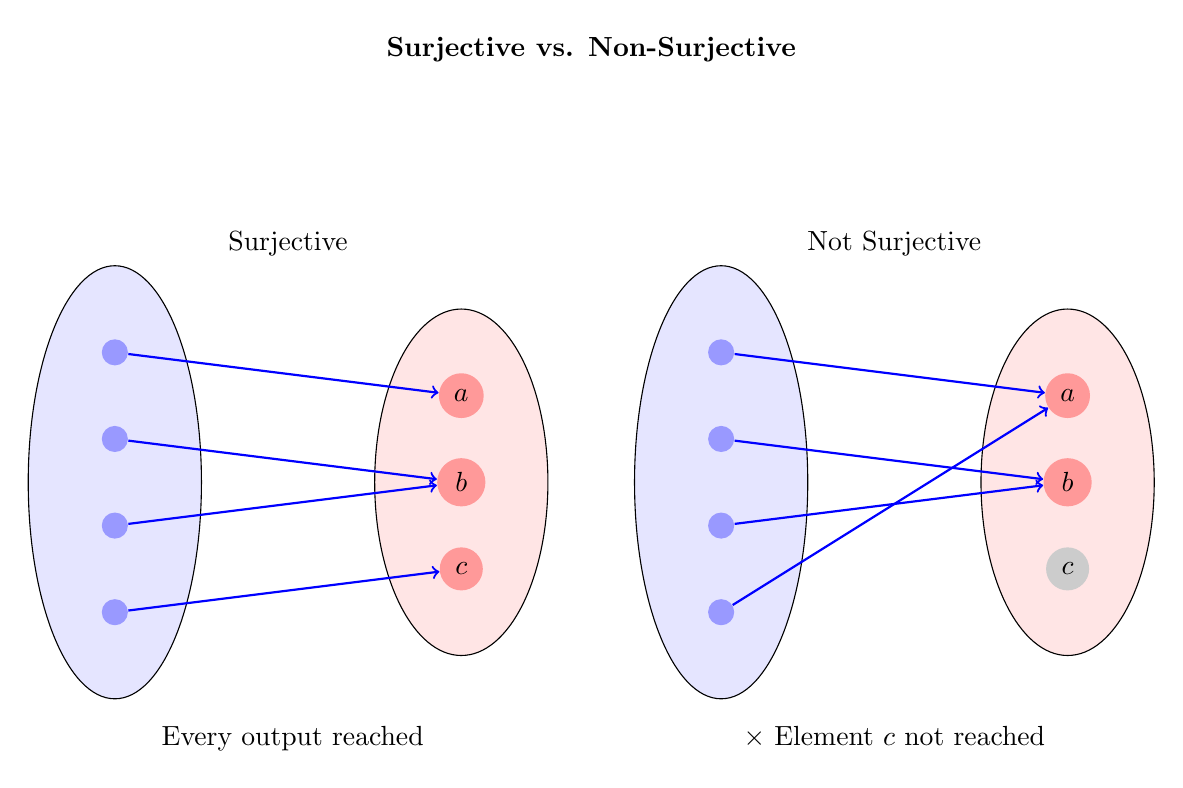
\begin{tikzpicture}[scale=1.1]
    \node at (5.5, 5) {\textbf{Surjective vs. Non-Surjective}};
    
    % Surjective
    \begin{scope}[shift={(0,0)}]
        \draw[fill=blue!10] (0,0) ellipse (1cm and 2.5cm);
        \draw[fill=red!10] (4,0) ellipse (1cm and 2cm);
        \node[above] at (2,2.5) {Surjective};
        
        \node[circle, fill=blue!40] (a1) at (0,1.5) {};
        \node[circle, fill=blue!40] (a2) at (0,0.5) {};
        \node[circle, fill=blue!40] (a3) at (0,-0.5) {};
        \node[circle, fill=blue!40] (a4) at (0,-1.5) {};
        
        \node[circle, fill=red!40] (b1) at (4,1) {$a$};
        \node[circle, fill=red!40] (b2) at (4,0) {$b$};
        \node[circle, fill=red!40] (b3) at (4,-1) {$c$};
        
        \draw[->, thick, blue] (a1) -- (b1);
        \draw[->, thick, blue] (a2) -- (b2);
        \draw[->, thick, blue] (a3) -- (b2);
        \draw[->, thick, blue] (a4) -- (b3);
        
        \node[below] at (2, -2.7) {$\checkmark$ Every output reached};
    \end{scope}
    
    % Non-surjective
    \begin{scope}[shift={(7,0)}]
        \draw[fill=blue!10] (0,0) ellipse (1cm and 2.5cm);
        \draw[fill=red!10] (4,0) ellipse (1cm and 2cm);
        \node[above] at (2,2.5) {Not Surjective};
        
        \node[circle, fill=blue!40] (a1) at (0,1.5) {};
        \node[circle, fill=blue!40] (a2) at (0,0.5) {};
        \node[circle, fill=blue!40] (a3) at (0,-0.5) {};
        \node[circle, fill=blue!40] (a4) at (0,-1.5) {};
        
        \node[circle, fill=red!40] (b1) at (4,1) {$a$};
        \node[circle, fill=red!40] (b2) at (4,0) {$b$};
        \node[circle, fill=gray!40] (b3) at (4,-1) {$c$};
        
        \draw[->, thick, blue] (a1) -- (b1);
        \draw[->, thick, blue] (a2) -- (b2);
        \draw[->, thick, blue] (a3) -- (b2);
        \draw[->, thick, blue] (a4) -- (b1);
        
        \node[below] at (2, -2.7) {$\times$ Element $c$ not reached};
    \end{scope}
\end{tikzpicture}
\end{center}

\begin{theorem}[Surjectivity Test]
To prove $f: A \to B$ is surjective:

\textbf{Start with:} An arbitrary $y \in B$

\textbf{Goal:} Find (or construct) $x \in A$ such that $f(x) = y$
\end{theorem}

\begin{example}[Proving Surjectivity]
Let $f: \mathbb{R} \to \mathbb{R}$ be defined by $f(x) = 3x + 7$.

\textbf{Claim}: $f$ is surjective.

\begin{proof}
Let $y \in \mathbb{R}$ be arbitrary. We need to find $x \in \mathbb{R}$ with $f(x) = y$.

Solve for $x$:
\begin{align*}
f(x) &= y \\
3x + 7 &= y \\
3x &= y - 7 \\
x &= \frac{y - 7}{3}
\end{align*}

Let $x = \frac{y - 7}{3}$. Then $x \in \mathbb{R}$ (since $y \in \mathbb{R}$) and:
\[f(x) = f\left(\frac{y-7}{3}\right) = 3 \cdot \frac{y-7}{3} + 7 = (y-7) + 7 = y\]

Therefore $f$ is surjective.
\end{proof}
\end{example}

\begin{example}[Non-Surjective Function]
Let $g: \mathbb{R} \to \mathbb{R}$ be defined by $g(x) = x^2$.

\textbf{Claim}: $g$ is NOT surjective.

\begin{proof}
Consider $y = -1 \in \mathbb{R}$ (codomain).

Is there $x \in \mathbb{R}$ with $g(x) = -1$?

We need $x^2 = -1$, but no real number squares to $-1$.

Therefore $-1 \notin \text{Im}(g)$, so $g$ is not surjective.
\end{proof}

\textbf{Note}: If we changed the codomain to $[0, \infty)$, then $g: \mathbb{R} \to [0, \infty)$ with $g(x) = x^2$ would be surjective!
\end{example}

\subsection{Bijective Functions (One-to-One Correspondences)}

\begin{intuition}
A bijective function is both injective and surjective---it pairs elements of $A$ and $B$ perfectly with no leftovers.

Think of assigning seats to students: if every student gets exactly one seat, and every seat has exactly one student, the assignment is bijective.

Bijections are the ``isomorphisms'' of set theory---they show that two sets have the same size.
\end{intuition}

\begin{definition}[Bijection]
A function $f: A \to B$ is \textbf{bijective} (or a \textbf{bijection}, or a \textbf{one-to-one correspondence}) if it is both:
\begin{enumerate}
    \item Injective (one-to-one)
    \item Surjective (onto)
\end{enumerate}
\end{definition}

egin{center}
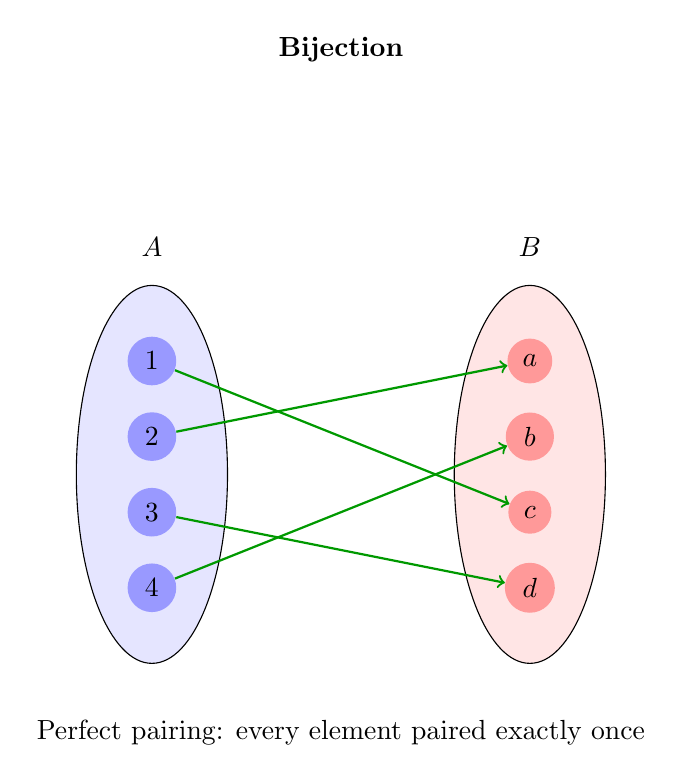
\begin{tikzpicture}[scale=1.2]
    \node at (2, 4.5) {\textbf{Bijection}};
    
    \draw[fill=blue!10] (0,0) ellipse (0.8cm and 2cm);
    \draw[fill=red!10] (4,0) ellipse (0.8cm and 2cm);
    
    \node[above] at (0,2.2) {$A$};
    \node[above] at (4,2.2) {$B$};
    
    \node[circle, fill=blue!40] (a1) at (0,1.2) {$1$};
    \node[circle, fill=blue!40] (a2) at (0,0.4) {$2$};
    \node[circle, fill=blue!40] (a3) at (0,-0.4) {$3$};
    \node[circle, fill=blue!40] (a4) at (0,-1.2) {$4$};
    
    \node[circle, fill=red!40] (b1) at (4,1.2) {$a$};
    \node[circle, fill=red!40] (b2) at (4,0.4) {$b$};
    \node[circle, fill=red!40] (b3) at (4,-0.4) {$c$};
    \node[circle, fill=red!40] (b4) at (4,-1.2) {$d$};
    
    \draw[->, thick, green!60!black] (a1) -- (b3);
    \draw[->, thick, green!60!black] (a2) -- (b1);
    \draw[->, thick, green!60!black] (a3) -- (b4);
    \draw[->, thick, green!60!black] (a4) -- (b2);
    
    \node[below] at (2, -2.5) {Perfect pairing: every element paired exactly once};
\end{tikzpicture}
\end{center}

\begin{theorem}[Characterization of Bijections]
$f: A \to B$ is bijective if and only if:
\[\forall y \in B, \exists! x \in A, f(x) = y\]

(For each output, there is exactly one input.)
\end{theorem}

\begin{proof}
($\Rightarrow$) Suppose $f$ is bijective.

Let $y \in B$. Since $f$ is surjective, $\exists x \in A$ with $f(x) = y$ (existence).

If there were another $x' \in A$ with $f(x') = y$, then $f(x) = f(x')$, which by injectivity implies $x = x'$ (uniqueness).

($\Leftarrow$) Suppose $\forall y \in B, \exists! x \in A, f(x) = y$.

\textbf{Surjective}: For any $y \in B$, the existence part gives $x$ with $f(x) = y$. $\checkmark$

\textbf{Injective}: Suppose $f(x_1) = f(x_2) = y$. By uniqueness, there's only one $x$ with $f(x) = y$, so $x_1 = x_2$. $\checkmark$

Therefore $f$ is bijective.
\end{proof}

\begin{example}[Bijections]
\begin{enumerate}
    \item $f: \mathbb{R} \to \mathbb{R}$, $f(x) = 3x + 7$ (linear with non-zero slope)
    
    \item $g: \mathbb{N} \to \mathbb{N}$, $g(n) = n + 1$ (successor function)
    
    \item $h: (0, 1) \to \mathbb{R}$, $h(x) = \tan\left(\pi\left(x - \frac{1}{2}\right)\right)$ (maps open interval to all reals)
\end{enumerate}
\end{example}

\section{Inverse Functions}

\begin{intuition}
If a function $f: A \to B$ is bijective, we can ``reverse'' it---for each output $y \in B$, there's exactly one input $x \in A$ that produced it.

The inverse function $f^{-1}: B \to A$ sends each output back to its unique input.
\end{intuition}

\begin{theorem}[Existence of Inverse]
A function $f: A \to B$ has an inverse function $f^{-1}: B \to A$ if and only if $f$ is bijective.
\end{theorem}

\begin{proof}
($\Rightarrow$) Suppose $f^{-1}: B \to A$ exists.

\textbf{Injective}: If $f(x_1) = f(x_2) = y$, then:
\[x_1 = f^{-1}(f(x_1)) = f^{-1}(y) = f^{-1}(f(x_2)) = x_2\]

\textbf{Surjective}: For any $y \in B$, let $x = f^{-1}(y) \in A$. Then $f(x) = f(f^{-1}(y)) = y$. $\checkmark$

($\Leftarrow$) Suppose $f$ is bijective.

Define $f^{-1}: B \to A$ by: for each $y \in B$, let $f^{-1}(y)$ be the unique $x \in A$ with $f(x) = y$.

(This $x$ exists and is unique because $f$ is bijective.)

We need to verify $f^{-1}$ is a function:
\begin{itemize}
    \item \textbf{Existence}: Every $y \in B$ has an image (by surjectivity of $f$)
    \item \textbf{Uniqueness}: Each $y$ has only one pre-image (by injectivity of $f$)
\end{itemize}

Therefore $f^{-1}$ exists.
\end{proof}

\begin{definition}[Inverse Function]
If $f: A \to B$ is bijective, the \textbf{inverse function} $f^{-1}: B \to A$ is defined by:
\[f^{-1}(y) = x \iff f(x) = y\]

Equivalently:
\begin{itemize}
    \item $f^{-1}(f(x)) = x$ for all $x \in A$
    \item $f(f^{-1}(y)) = y$ for all $y \in B$
\end{itemize}
\end{definition}

\begin{center}
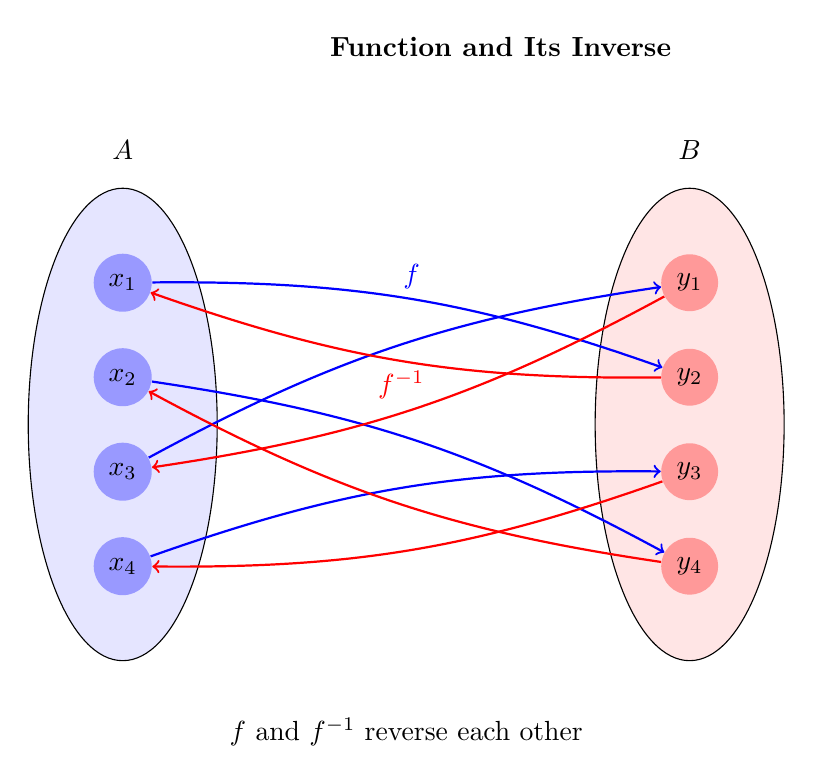
\begin{tikzpicture}[scale=1.2]
    \node at (4, 4) {\textbf{Function and Its Inverse}};
    
    \draw[fill=blue!10] (0,0) ellipse (1cm and 2.5cm);
    \draw[fill=red!10] (6,0) ellipse (1cm and 2.5cm);
    
    \node[above] at (0,2.7) {$A$};
    \node[above] at (6,2.7) {$B$};
    
    \node[circle, fill=blue!40] (a1) at (0,1.5) {$x_1$};
    \node[circle, fill=blue!40] (a2) at (0,0.5) {$x_2$};
    \node[circle, fill=blue!40] (a3) at (0,-0.5) {$x_3$};
    \node[circle, fill=blue!40] (a4) at (0,-1.5) {$x_4$};
    
    \node[circle, fill=red!40] (b1) at (6,1.5) {$y_1$};
    \node[circle, fill=red!40] (b2) at (6,0.5) {$y_2$};
    \node[circle, fill=red!40] (b3) at (6,-0.5) {$y_3$};
    \node[circle, fill=red!40] (b4) at (6,-1.5) {$y_4$};
    
    \draw[->, thick, blue, bend left=10] (a1) to node[above] {$f$} (b2);
    \draw[->, thick, blue, bend left=10] (a2) to (b4);
    \draw[->, thick, blue, bend left=10] (a3) to (b1);
    \draw[->, thick, blue, bend left=10] (a4) to (b3);
    
    \draw[->, thick, red, bend left=10] (b2) to node[below] {$f^{-1}$} (a1);
    \draw[->, thick, red, bend left=10] (b4) to (a2);
    \draw[->, thick, red, bend left=10] (b1) to (a3);
    \draw[->, thick, red, bend left=10] (b3) to (a4);
    
    \node[below] at (3, -3) {$f$ and $f^{-1}$ reverse each other};
\end{tikzpicture}
\end{center}

\begin{warning}
\textbf{Inverse Notation Ambiguity}

For general relations, $R^{-1} = \{(b, a) : (a, b) \in R\}$ always exists (just swap pairs).

But for functions, $f^{-1}$ as a \textit{function} only exists when $f$ is bijective!

Also: Don't confuse $f^{-1}(x)$ (inverse function) with $\frac{1}{f(x)}$ (reciprocal). These are completely different!
\end{warning}

\begin{example}[Computing Inverse]
Let $f: \mathbb{R} \to \mathbb{R}$ be $f(x) = 3x + 7$ (we proved this is bijective).

Find $f^{-1}$.

\begin{proof}[Solution]
We need to solve $y = f(x)$ for $x$ in terms of $y$:
\begin{align*}
y &= 3x + 7 \\
y - 7 &= 3x \\
x &= \frac{y - 7}{3}
\end{align*}

Therefore: $f^{-1}(y) = \frac{y - 7}{3}$.

Or, using $x$ as the variable: $f^{-1}(x) = \frac{x - 7}{3}$.

\textbf{Check}:
\begin{align*}
f(f^{-1}(x)) &= f\left(\frac{x-7}{3}\right) = 3 \cdot \frac{x-7}{3} + 7 = x \quad $\checkmark$ \\
f^{-1}(f(x)) &= f^{-1}(3x + 7) = \frac{(3x+7) - 7}{3} = \frac{3x}{3} = x \quad $\checkmark$
\end{align*}
\end{proof}
\end{example}

\section{Images and Preimages of Sets}

Functions don't just map elements to elements; they also map \textit{subsets} to \textit{subsets}.

\begin{definition}[Image of a Set]
Let $f: A \to B$ be a function and $S \subseteq A$. The \textbf{image} of $S$ under $f$ is:
\[f[S] := \{f(x) : x \in S\} = \{y \in B : \exists x \in S, f(x) = y\}\]
\end{definition}

\begin{definition}[Preimage of a Set]
Let $f: A \to B$ be a function and $T \subseteq B$. The \textbf{preimage} (or inverse image) of $T$ under $f$ is:
\[f^{-1}[T] := \{x \in A : f(x) \in T\}\]
\end{definition}

\begin{warning}
\textbf{The Symbol $f^{-1}$ Overload}

We use the symbol $f^{-1}$ in two different ways:
\begin{enumerate}
    \item \textbf{Inverse Function}: $f^{-1}(y)$ (Exists only if $f$ is bijective)
    \item \textbf{Preimage}: $f^{-1}[T]$ (Exists for \textit{any} function)
\end{enumerate}

When $f$ is bijective, these concepts align: $f^{-1}[\{y\}] = \{f^{-1}(y)\}$.
But if $f$ is not bijective, $f^{-1}[T]$ is a set, while the inverse function $f^{-1}$ does not exist.
\end{warning}

\begin{example}
Let $f: \mathbb{R} \to \mathbb{R}$ be $f(x) = x^2$.
\begin{itemize}
    \item Image of interval: $f[[1, 2]] = [1, 4]$.
    \item Preimage of singleton: $f^{-1}[\{4\}] = \{-2, 2\}$.
    \item Preimage of interval: $f^{-1}[[1, 4]] = [-2, -1] \cup [1, 2]$.
    \item Preimage of negative numbers: $f^{-1}[[-5, -1]] = \emptyset$.
\end{itemize}
\end{example}

\begin{theorem}[Properties of Image and Preimage]
For any function $f: A \to B$:
\begin{enumerate}
    \item \textbf{Preimage preserves set operations}:
    \begin{align*}
    f^{-1}[T_1 \cup T_2] &= f^{-1}[T_1] \cup f^{-1}[T_2] \\
    f^{-1}[T_1 \cap T_2] &= f^{-1}[T_1] \cap f^{-1}[T_2] \\
    f^{-1}[B \setminus T] &= A \setminus f^{-1}[T]
    \end{align*}
    
    \item \textbf{Image preserves unions, but NOT intersections}:
    \begin{align*}
    f[S_1 \cup S_2] &= f[S_1] \cup f[S_2] \\
    f[S_1 \cap S_2] &\subseteq f[S_1] \cap f[S_2] \quad \text{(Equality holds if $f$ is injective)}
    \end{align*}
\end{enumerate}
\end{theorem}

\section{Composition of Functions}

\begin{intuition}
Composition means ``do one function, then another.''

If $f: A \to B$ transforms $A$-elements into $B$-elements, and $g: B \to C$ transforms $B$-elements into $C$-elements, then $g \circ f: A \to C$ does both transformations in sequence.

Think of assembly lines: raw material → intermediate product → final product.
\end{intuition}

\begin{definition}[Composition]
Let $f: A \to B$ and $g: B \to C$ be functions. The \textbf{composition} $g \circ f: A \to C$ is defined by:
\[(g \circ f)(x) = g(f(x)) \quad \text{for all } x \in A\]
\end{definition}

\begin{center}
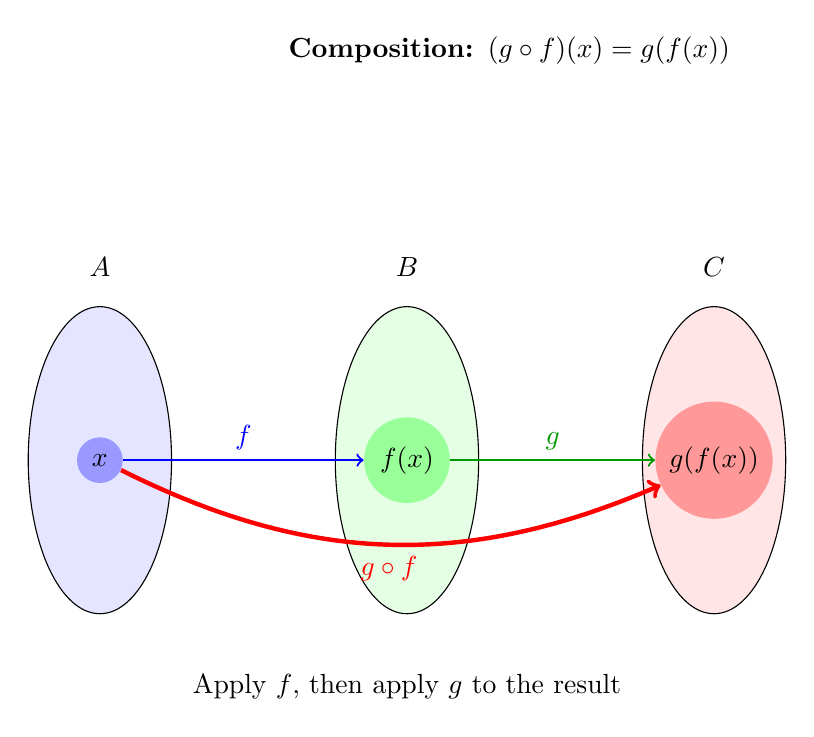
\begin{tikzpicture}[scale=1.3]
    \node at (4, 4) {\textbf{Composition: $(g \circ f)(x) = g(f(x))$}};
    
    % Sets
    \draw[fill=blue!10] (0,0) ellipse (0.7cm and 1.5cm);
    \node[above] at (0,1.7) {$A$};
    
    \draw[fill=green!10] (3,0) ellipse (0.7cm and 1.5cm);
    \node[above] at (3,1.7) {$B$};
    
    \draw[fill=red!10] (6,0) ellipse (0.7cm and 1.5cm);
    \node[above] at (6,1.7) {$C$};
    
    % Elements
    \node[circle, fill=blue!40] (x) at (0,0) {$x$};
    \node[circle, fill=green!40] (fx) at (3,0) {$f(x)$};
    \node[circle, fill=red!40] (gfx) at (6,0) {$g(f(x))$};
    
    % Arrows
    \draw[->, thick, blue] (x) -- (fx) node[midway, above] {$f$};
    \draw[->, thick, green!60!black] (fx) -- (gfx) node[midway, above] {$g$};
    \draw[->, ultra thick, red, bend right=25] (x) to node[below] {$g \circ f$} (gfx);
    
    \node[below] at (3, -2) {Apply $f$, then apply $g$ to the result};
\end{tikzpicture}
\end{center}

\begin{warning}
\textbf{Order Matters!}

Composition is generally \textbf{not commutative}: $g \circ f \neq f \circ g$

In fact, $f \circ g$ might not even be defined (if codomain of $g$ $\neq$ domain of $f$).

When writing $(g \circ f)(x)$, read right-to-left: apply $f$ first, then $g$.
\end{warning}

\begin{example}[Composition]
Let $f: \mathbb{R} \to \mathbb{R}$, $f(x) = x^2$, and $g: \mathbb{R} \to \mathbb{R}$, $g(x) = x + 1$.

Then:
\begin{itemize}
    \item $(g \circ f)(x) = g(f(x)) = g(x^2) = x^2 + 1$
    \item $(f \circ g)(x) = f(g(x)) = f(x + 1) = (x + 1)^2 = x^2 + 2x + 1$
\end{itemize}

Note: $(g \circ f)(x) \neq (f \circ g)(x)$ in general.
\end{example}

\subsection{Properties of Composition}

\begin{theorem}[Composition is Associative]
Let $f: A \to B$, $g: B \to C$, $h: C \to D$. Then:
\[h \circ (g \circ f) = (h \circ g) \circ f\]
\end{theorem}

\begin{proof}
We show both functions have the same domain, codomain, and give the same output for every input.

\textbf{Domain and Codomain}: Both are functions from $A$ to $D$. $\checkmark$

\textbf{Outputs}: For any $x \in A$:
\begin{align*}
[h \circ (g \circ f)](x) &= h((g \circ f)(x)) \\
&= h(g(f(x))) \\
&= (h \circ g)(f(x)) \\
&= [(h \circ g) \circ f](x)
\end{align*}

Since they agree on all $x \in A$, the functions are equal.
\end{proof}

\begin{remark}
Associativity means we can write $h \circ g \circ f$ without ambiguity---no matter how we parenthesize, the result is the same.

This is crucial for defining powers: $f^n = f \circ f \circ \cdots \circ f$ (n times).
\end{remark}

\begin{theorem}[Identity Functions]
For any set $A$, define the \textbf{identity function} $\text{id}_A: A \to A$ by:
\[\text{id}_A(x) = x \quad \text{for all } x \in A\]

For any function $f: A \to B$:
\[f \circ \text{id}_A = f = \text{id}_B \circ f\]
\end{theorem}

\begin{proof}
For any $x \in A$:
\[(f \circ \text{id}_A)(x) = f(\text{id}_A(x)) = f(x)\]
\[(\text{id}_B \circ f)(x) = \text{id}_B(f(x)) = f(x)\]

Therefore both compositions equal $f$.
\end{proof}

\begin{theorem}[Composition Preserves Properties]
\begin{enumerate}
    \item If $f: A \to B$ and $g: B \to C$ are both injective, then $g \circ f$ is injective.
    
    \item If $f$ and $g$ are both surjective, then $g \circ f$ is surjective.
    
    \item If $f$ and $g$ are both bijective, then $g \circ f$ is bijective.
\end{enumerate}
\end{theorem}

\begin{proof}
\textbf{(1) Injectivity}:

Suppose $f$ and $g$ are injective. Let $x_1, x_2 \in A$ and suppose $(g \circ f)(x_1) = (g \circ f)(x_2)$.

Then:
\begin{align*}
g(f(x_1)) &= g(f(x_2)) \\
\implies f(x_1) &= f(x_2) \quad \text{($g$ injective)} \\
\implies x_1 &= x_2 \quad \text{($f$ injective)}
\end{align*}

Therefore $g \circ f$ is injective. $\checkmark$

\textbf{(2) Surjectivity}:

Suppose $f$ and $g$ are surjective. Let $z \in C$.

Since $g$ is surjective, $\exists y \in B$ with $g(y) = z$.

Since $f$ is surjective, $\exists x \in A$ with $f(x) = y$.

Therefore:
\[(g \circ f)(x) = g(f(x)) = g(y) = z\]

So $g \circ f$ is surjective. $\checkmark$

\textbf{(3)} Follows from (1) and (2).
\end{proof}

\begin{theorem}[Inverse of Composition]
If $f: A \to B$ and $g: B \to C$ are both bijections, then:
\[(g \circ f)^{-1} = f^{-1} \circ g^{-1}\]

(The inverse of a composition is the composition of inverses in reverse order.)
\end{theorem}

\begin{proof}
We show $(f^{-1} \circ g^{-1}) \circ (g \circ f) = \text{id}_A$ and $(g \circ f) \circ (f^{-1} \circ g^{-1}) = \text{id}_C$.

For any $x \in A$:
\begin{align*}
[(f^{-1} \circ g^{-1}) \circ (g \circ f)](x) &= f^{-1}(g^{-1}(g(f(x)))) \\
&= f^{-1}(f(x)) \quad \text{($g^{-1} \circ g = \text{id}_B$)} \\
&= x \quad \text{($f^{-1} \circ f = \text{id}_A$)}
\end{align*}

Similarly for the other composition. Therefore $f^{-1} \circ g^{-1}$ is the inverse of $g \circ f$.
\end{proof}

\section{Special Classes of Functions}

\subsection{Constant Functions}

\begin{definition}[Constant Function]
A function $f: A \to B$ is \textbf{constant} if there exists $b \in B$ such that:
\[f(x) = b \quad \text{for all } x \in A\]
\end{definition}

\begin{remark}
Constant functions are:
\begin{itemize}
    \item \textbf{Never injective} (unless $|A| \leq 1$): all inputs map to the same output
    \item \textbf{Never surjective} (unless $|B| = 1$): only one element of $B$ is reached
\end{itemize}
\end{remark}

\subsection{Inclusion Maps}

\begin{definition}[Inclusion Map]
Let $A \subseteq B$. The \textbf{inclusion map} $\iota: A \to B$ is defined by:
\[\iota(x) = x \quad \text{for all } x \in A\]
\end{definition}

\begin{theorem}
Every inclusion map is injective.

An inclusion map $\iota: A \to B$ is surjective if and only if $A = B$.
\end{theorem}

\subsection{Restrictions and Extensions}

\begin{definition}[Restriction]
Let $f: A \to B$ be a function and $S \subseteq A$. The \textbf{restriction} of $f$ to $S$, denoted $f|_S: S \to B$, is:
\[f|_S(x) = f(x) \quad \text{for all } x \in S\]
\end{definition}

\begin{example}
Let $f: \mathbb{R} \to \mathbb{R}$, $f(x) = x^2$.

The restriction $f|_{[0, \infty)}: [0, \infty) \to \mathbb{R}$ is injective (even though $f$ is not).
\end{example}

\section{Functions and Cardinality}

\begin{keyidea}
Functions provide a rigorous way to compare sizes of sets:

\begin{itemize}
    \item $|A| \leq |B|$ $\iff$ there exists an injection $f: A \to B$
    
    \item $|A| = |B|$ $\iff$ there exists a bijection $f: A \to B$
\end{itemize}

This works even for infinite sets! We'll explore this fully in the Cardinality chapter.
\end{keyidea}

\begin{theorem}[Pigeonhole Principle - Finite Version]
If $f: A \to B$ is a function between finite sets with $|A| > |B|$, then $f$ is not injective.
\end{theorem}

\begin{proof}
Suppose $f$ were injective. Then distinct elements of $A$ map to distinct elements of $B$.

Since $|A| > |B|$, there are more elements in $A$ than in $B$, so we run out of elements in $B$---contradiction.
\end{proof}

\begin{remark}
This is the ``pigeonhole principle'': if you have more pigeons than pigeonholes, at least one hole contains multiple pigeons.
\end{remark}

\section{Looking Forward}

Functions are the most important concept in mathematics:
\begin{itemize}
    \item \textbf{Algebra}: Homomorphisms preserve structure
    \item \textbf{Topology}: Continuous functions preserve nearness
    \item \textbf{Category Theory}: Morphisms generalize functions
    \item \textbf{Analysis}: Limits, derivatives, integrals are all defined via functions
\end{itemize}

Next, we'll use bijections to compare sizes of infinite sets---discovering that not all infinities are equal!

\begin{center}
\begin{tikzpicture}[scale=1.1]
    \node[rectangle, draw, fill=yellow!20, text width=10cm, align=center] at (5,0) {
    \textbf{The Hierarchy of Structure} \\[0.3cm]
    Relations ⊃ Functions ⊃ Injections ⊃ Bijections \\[0.2cm]
    Each subset adds more constraints, more structure, more power.
    };
\end{tikzpicture}
\end{center}
